\documentclass[10pt]{article}
\usepackage[a4paper,margin=18mm,top=20mm,bottom=18mm,headsep=5mm,footskip=8mm]{geometry}
\usepackage{fontspec}
\setmainfont{Carlito}
\setmonofont{DejaVu Sans Mono}[Scale=0.85]
\usepackage{xcolor}
\definecolor{ink}{HTML}{1F2A44}
\usepackage{graphicx,tabularx,booktabs,array,enumitem,fancyhdr,lastpage}
\usepackage{pdflscape}
\newenvironment{claimpage}{}{}
\color{ink}
\pagestyle{fancy}\fancyhf{}
\renewcommand{\headrulewidth}{0pt}
\fancyhead[L]{\footnotesize\color{ink}CasePath paper rebuild: gate 1 (13 November 2026)}
\fancyfoot[C]{\footnotesize\color{ink}\thepage\ of \pageref*{LastPage}}
\setlength{\parindent}{0pt}\setlength{\parskip}{3pt}
\newcommand{\code}[1]{\texttt{#1}}
\newcommand{\doctitle}[1]{{\large\bfseries #1\par}\vspace{2pt}}
\usepackage{needspace}
\newcommand{\sect}[1]{\needspace{5\baselineskip}\vspace{3pt}{\bfseries #1\par}\vspace{1pt}}
\setlist{nosep,leftmargin=1.4em}
\setlength{\aboverulesep}{1pt}\setlength{\belowrulesep}{1pt}
\usepackage[hidelinks]{hyperref}
\begin{document}

\newgeometry{margin=14mm,top=17mm,bottom=15mm,headsep=4mm,footskip=7mm}\begin{claimpage}\fontsize{9}{10.8}\selectfont\setlength{\tabcolsep}{3.5pt}\renewcommand{\arraystretch}{1.0}\renewcommand{\sect}[1]{\vspace{3pt}{\bfseries #1\par}\vspace{1pt}}\setlength{\parskip}{2pt}
\doctitle{Claim sheet (gate 1, draft for Navish, 2026-11-13)}
\textbf{Thesis.} Models read and quote; code decides; what the file leaves open becomes a held request with one question.

Every claim below names its figure, the evidence that exists today, and the evidence that must be produced. “Exists” means stored and reproducible; the numbers come from the figure drafts' data files. Study 3's figures are for its 96 sealed tenancy claims unless theft is named.

\sect{Question 1. What happens to a fact the file leaves open?}
\begin{tabularx}{\linewidth}{>{\raggedright\arraybackslash}p{0.8em}>{\hsize=0.95\hsize\raggedright\arraybackslash}X>{\raggedright\arraybackslash}p{4.2em}>{\hsize=1.25\hsize\raggedright\arraybackslash}X>{\hsize=0.8\hsize\raggedright\arraybackslash}X}\toprule
\textbf{\#} & \textbf{Claim} & \textbf{Figure} & \textbf{Exists today} & \textbf{Must be produced}\\\midrule
1 & With only “true” and “false“, a reading must take one branch: it asks for that branch's documents too early or drops the other's. A third value lets code request what both branches need and hold the rest. & 3 & Formal: follows from the definition of the workflow; shown on a real fragment of a public rule set. & Nothing.\\
2 & One sentence in the file decides one line of the checklist, and the line can be followed back to the quoted words. & 1, 2 & One stored pair of claims, drawn as it is. \textbf{Not true in general yet:} in 144 stored theft pair-runs the core changed only the governed line in 12; in 130 another line moved too, because readings of other facts differ between runs. & A fix that makes the same text give the same checklist. Then sealed twins in Study 4: two files one sentence apart, exact and collateral changes counted for every design.\\
3 & Of 100 requests that depend on an open fact, CasePath holds almost all, each with the right question. A prompt that is not told to hold asks for half of them too early. A prompt that is told holds them too, but then also holds or drops requests the file settles. & 4 & On the cost-efficient model the core holds 99.6 of 100, the plain prompt 48, the prompt that may hold 97 (86 documents in 32 claims). Of 100 settled requests the core gets 96 right, the prompt that may hold 90 (481 documents). \textbf{Lost today:} on the frontier model the core holds 87, the prompt that may hold 98. The prompt that may hold ran after the test. & Study 4, with needless holds counted as errors.\\
\bottomrule\end{tabularx}

\sect{Question 2. Does CasePath beat the strongest prompt as cases get real?}
\begin{tabularx}{\linewidth}{>{\raggedright\arraybackslash}p{0.8em}>{\hsize=0.95\hsize\raggedright\arraybackslash}X>{\raggedright\arraybackslash}p{4.2em}>{\hsize=1.25\hsize\raggedright\arraybackslash}X>{\hsize=0.8\hsize\raggedright\arraybackslash}X}\toprule
\textbf{\#} & \textbf{Claim} & \textbf{Figure} & \textbf{Exists today} & \textbf{Must be produced}\\\midrule
4 & CasePath's error holds its level as files get longer, rule catalogues larger and open facts more frequent; the strongest prompt's error rises. & 5, main table & \textbf{Nothing that supports this.} Study 3's files have 77 to 320 words. The public-rule benchmark has run no baseline. Today a prompt told the hold rules ties CasePath on tenancy (0.35 against 0.31 strict errors per claim) and beats it on claims that deny their defining event (0.00 against 0.61 on the frontier model). & Three fixes on development data, then Study 4 on fresh sealed files. Every cell is shown, won or lost.\\
5 & The lead does not cost many times a prompt, and the same file gives the same checklist when run again. & 7 & The core costs about 4 times the prompt that may hold on the same model (USD 0.0030 against 0.0007 per claim) for 0.73 against 0.89 errors; on the frontier model it costs 3.4 times as much and errs more (0.70 against 0.58). As tested it would cost about 40 times that prompt on a 2,500-word file (extrapolated). The same checklist in all three stored runs: 70 of 96 claims for the core. & Fixes to cost (the file read once and reused; supplied documents judged in one call; one reading where it settles the fact). Ten runs of the same file in Study 4.\\
\bottomrule\end{tabularx}

\sect{Question 3. What does an organisation gain when its rules change, or when it adds a kind of claim?}
\begin{tabularx}{\linewidth}{>{\raggedright\arraybackslash}p{0.8em}>{\hsize=0.95\hsize\raggedright\arraybackslash}X>{\raggedright\arraybackslash}p{4.2em}>{\hsize=1.25\hsize\raggedright\arraybackslash}X>{\hsize=0.8\hsize\raggedright\arraybackslash}X}\toprule
\textbf{\#} & \textbf{Claim} & \textbf{Figure} & \textbf{Exists today} & \textbf{Must be produced}\\\midrule
6 & After a rule edit, code recomputes every stored checklist with no model call and changes only the lines the edit reaches. A prompt must read every file again. & 6 & Replay of stored readings under one edited rule: 15 of 421 lines changed in 56 theft files, 14 as the edit requires, no model call. The prompt's side is not measured. & Rule-change experiment: a set of edits; exact changes, collateral changes and model calls for every design. An edit that adds a new fact costs CasePath readings of that fact only; this is measured too.\\
7 & A new kind of claim is added from public text in six steps by a session that has not seen the system. & table & Three regimes were built this way (177 cited rules); effort was not recorded; first use found 39 wording errors, since repaired. & A fresh session adds a fourth regime; effort is recorded; its sealed result enters Study 4.\\
8 & The system is small: a workflow is a data file and a new rule is one line; routing; several attachments and scans; presumptions; Knowledge from handler corrections, replayed without a model. & one listing or frame each & In the product at the tested commit. & Frames on synthetic cases, requested from the product session.\\
\bottomrule\end{tabularx}

\sect{What the paper does not claim}
No claim rests on the hackathon dossiers or the expert study. Studies 1 and 2, the commit timeline and the deviations list go to the supplement. If a cell of the main table is lost after the fixes, the table shows it and one sentence says why.

\end{claimpage}\clearpage\restoregeometry
{\large\bfseries Figure 1. One changed sentence\par}\vspace{6pt}
{\small The reader should see that replacing the one sentence that states a fact with one that leaves it open changes one checklist line from “requested now” to “held, with one question“, and leaves every other need in the same place and state, because that line is the only need whose rule names the fact the sentence leaves open.\par}\vspace{8pt}
\begin{center}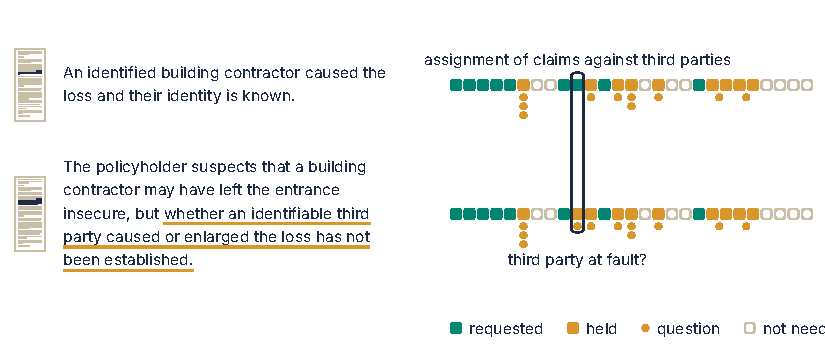
\includegraphics[width=5.5in]{../figures/f1/f1.pdf}\end{center}
\vspace{2pt}\begin{center}\begin{minipage}{5.5in}
One stored run: two claims, one sentence apart; the second leaves the third party's role open. Of 27 needs, one turns from requested to held. Each dot: one question per open fact a held line awaits. Nothing else changed in 12 of 144 stored pair-runs.\par\vspace{8pt}
{\footnotesize \textbf{Status:} Measured: page miniatures, the two sentences, the 27 squares per claim and their states, the question circles (attachment formal, from required\_when). Formal: rails linking the same need; ink rail and frame on d15. Not yet measured: no element.\par\vspace{3pt}
\textbf{Rejected construction:} b, one page and one fused strip: it shows a computed diff, not the two stored records; it draws one file for two and drops the questions.\par}
\end{minipage}\end{center}
\clearpage
{\large\bfseries Figure 2. The journey of one sentence\par}\vspace{6pt}
{\small The reader should see that the model contributes only quoted words and a verdict per reading, and that the quotation check, the agreement of the three readings, the fact's value deciding its rule, and the checklist line are computed by code, because the checklist line can be followed back across the one rule, along three lines, to the words each reading quoted.\par}\vspace{8pt}
\begin{center}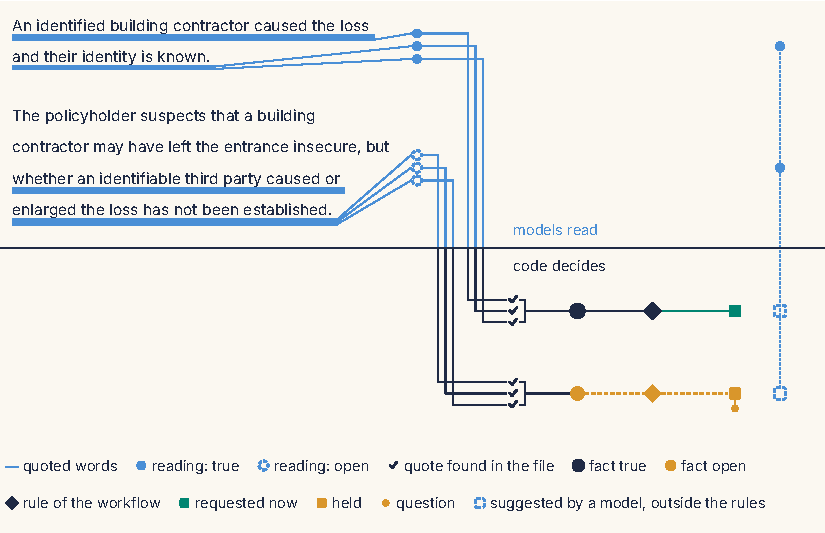
\includegraphics[width=5.5in]{../figures/f2/f2.pdf}\end{center}
\vspace{2pt}\begin{center}\begin{minipage}{5.5in}
One sentence, stated (top) or left open (bottom). Three readings each quote the file's words. Below the line, code checks each quotation, admits a value only when all three agree, and the fact decides its one rule: request now, or hold with one question.\par\vspace{8pt}
{\footnotesize \textbf{Status:} Measured: sentences and words, quotation underlines, reading marks, ticks (recomputed by substring), the fact’s value, the checklist line. Formal: agreement bracket (team.py rule, measured inputs), diamond node, outgoing edge. Schematic: horizontal positions. Not yet measured: no element.\par\vspace{3pt}
\textbf{Rejected construction:} a, one lane, the open sentence alone: no partner; amber can’t be read as a change without the stated lane.\par}
\end{minipage}\end{center}
\clearpage
{\large\bfseries Figure 3. Why “open” needs its own value\par}\vspace{6pt}
{\small The reader should see that a reading that may only say true or false must send the case down one branch, and so either asks for the police consent too early (true) or drops it (false), while the value “open” lets code request the list of stolen items, which both branches need after they rejoin, and hold only the police consent, with one question, because the two branches of “traces altered?” meet again before the list is needed.\par}\vspace{8pt}
\begin{center}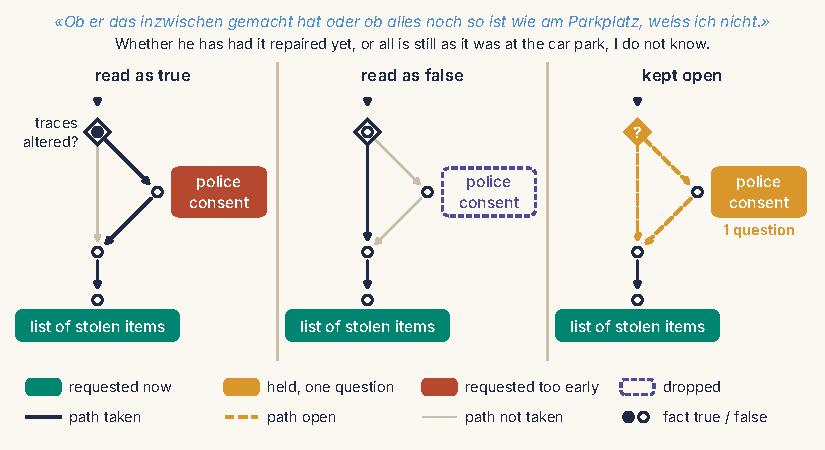
\includegraphics[width=5.5in]{../figures/f3/f3.pdf}\end{center}
\vspace{2pt}\begin{center}\begin{minipage}{5.5in}
The same file, read three ways. Read as true, the police consent is asked too early; read as false, it is dropped. Kept open, both branches stay possible: code still requests the list of stolen items, needed after they rejoin, and holds only the consent, with one question.\par\vspace{8pt}
{\footnotesize \textbf{Status:} Formal: follows from the definitions, computed by the product’s own evaluator, on a real instance. Measured: all three stored readings answer open, quoting the sentence. Schematic simplification: a\_instruction contracted. Not yet measured: no element.\par\vspace{3pt}
\textbf{Rejected construction:} b, the fragment once beside a 2 × 3 matrix: the mechanism (branch walked, rejoin) is not visible per reading; it hides the cause.\par}
\end{minipage}\end{center}
\clearpage
{\large\bfseries Figure 4. The fate of 100 open facts\par}\vspace{6pt}
{\small The reader should see that of 100 requests whose need hangs on a fact the file leaves open, CasePath and the prompts told they may hold keep about 97 waiting with a question, while the Study 3 prompts ask for half or more too early; and that CasePath pays with holds the file does not need (mostly where the claim denies its defining event), because a hold is the right fate only where the need depends on the open fact, so the partner panel must show what each design does where the file settles the need.\par}\vspace{8pt}
\begin{center}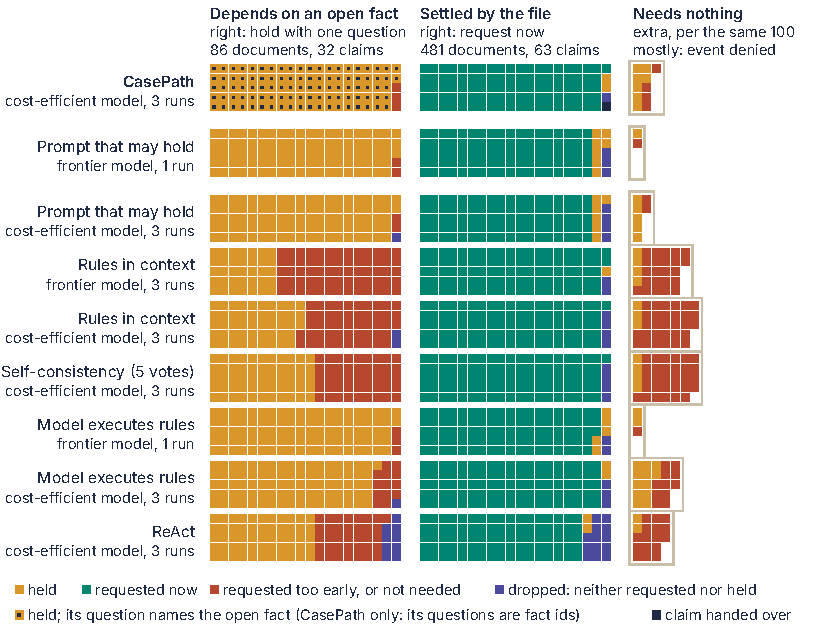
\includegraphics[width=5.5in]{../figures/f4/f4.pdf}\end{center}
\vspace{2pt}\begin{center}\begin{minipage}{5.5in}
Where the need hangs on an open fact, CasePath's core and prompts allowed to hold keep nearly all requests waiting; earlier prompts ask early. CasePath's price: holds where nothing is needed. 86 open, 481 settled documents, 1 to 3 runs; CasePath's question names the fact.\par\vspace{8pt}
{\footnotesize \textbf{Status:} Measured: every mark. Formal: grouping into 5 × 20 grids and largest-remainder rounding. Not yet measured: free-text questions of the other designs (no registered scorer).\par\vspace{3pt}
\textbf{Rejected construction:} b, aligned error bars: three different x-scales make 3 settled errors look like 30 open ones, and the right share disappears from view.\par}
\end{minipage}\end{center}
\clearpage
{\large\bfseries Figure 5. As cases get real\par}\vspace{6pt}
{\small The reader should see that stored data measure each design's error at one point on each of the three axes (files of 77 to 367 words, one catalogue of three claim types, one third of files with an open fact), and that the planned ranges are empty, because the registered test (Study 4) has not run, so whether a design that reads one fact at a time and decides in code holds its level where a single prompt does not is still unanswered.\par}\vspace{8pt}
\begin{center}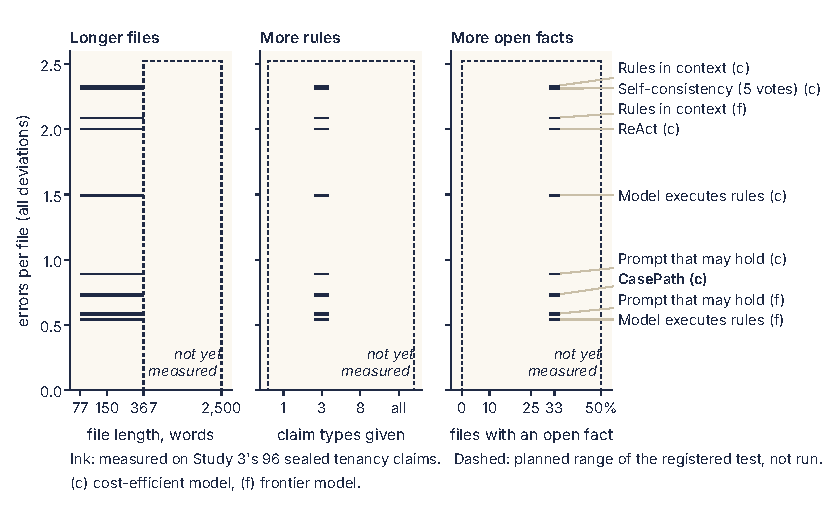
\includegraphics[width=5.5in]{../figures/f5/f5.pdf}\end{center}
\vspace{2pt}\begin{center}\begin{minipage}{5.5in}
Study 3 measures each design at one point per axis: 77 to 367 words (message plus attachments; bracket), one catalogue of three claim types, a third of files with an open fact. The registered test's ranges (dashed) are empty: the question is unanswered.\par\vspace{8pt}
{\footnotesize \textbf{Status:} Measured: ink levels (Study 3 sealed tenancy). Not yet measured: the dashed regions (planned ranges of the registered test).\par\vspace{3pt}
\textbf{Rejected construction:} a, tercile lines: a steep “length effect” that is the denied-event claims.\par}
\end{minipage}\end{center}
\clearpage
{\large\bfseries Figure 6. A rule changes\par}\vspace{6pt}
{\small The reader should see that after one edited rule line, code recomputes every stored checklist of the regime from the stored readings with no model call and changes only the lines the edit reaches, while a prompt must read every file again, because CasePath stores one reading per fact and the rules are data.\par}\vspace{8pt}
\begin{center}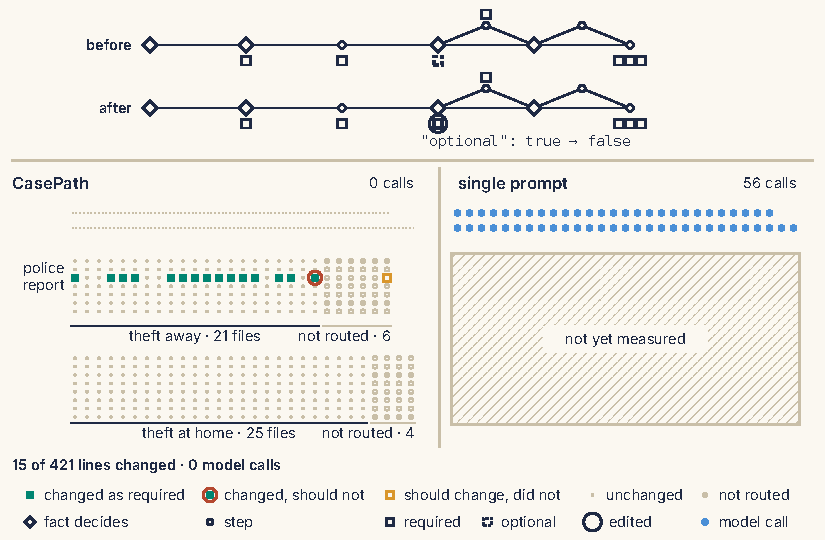
\includegraphics[width=5.5in]{../figures/f6/f6.pdf}\end{center}
\vspace{2pt}\begin{center}\begin{minipage}{5.5in}
One line made the police report required. From stored readings, code recomputed all 56 checklists, no model call; only police-report lines changed. One extra request: a report on file, finding rejected; one missed hold: a file never routed. A prompt reads every file again.\par\vspace{8pt}
{\footnotesize \textbf{Status:} Measured (left): stored replay, changed and collateral lines, 0 model calls. Formal (right): the prompt reads every file again, 56 calls. Not yet measured: the prompt’s changed lines (hatched frame).\par\vspace{3pt}
\textbf{Rejected construction:} b, a before→after transition table: loses which file and which document changed, and the graph.\par}
\end{minipage}\end{center}
\clearpage
{\large\bfseries Figure 7. The price\par}\vspace{6pt}
{\small The reader should see that on Study 3's tenancy claims the full product costs about 20 times the same-model prompt and twice the frontier prompt that may hold, which has fewer deviations; that its checklist-only core costs 4 times the prompt for the same error; and how often the same file gives the same checklist again, because a lower error that costs many times more, or changes from run to run, is not useful.\par}\vspace{8pt}
\begin{center}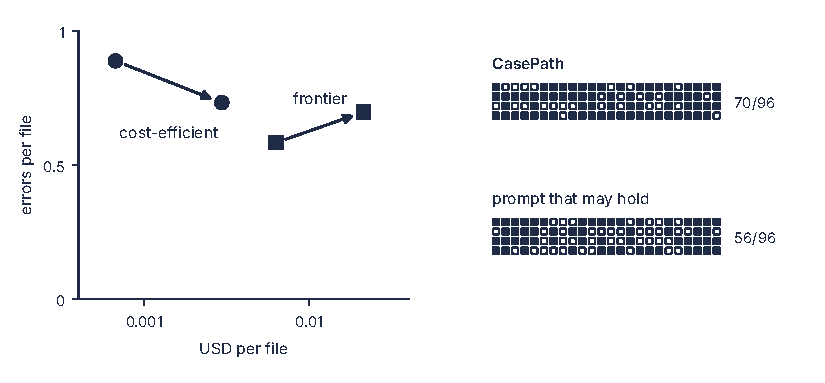
\includegraphics[width=5.5in]{../figures/f7/f7.pdf}\end{center}
\vspace{2pt}\begin{center}\begin{minipage}{5.5in}
On Study 3's claims CasePath's core costs four times the same-model prompt that may hold, with fewer deviations; the frontier prompt errs less at twice the cost. One reading errs less than three. Run again, 5 to 8\% of lines change; three runs, not ten.\par\vspace{8pt}
{\footnotesize \textbf{Status:} Measured: all marks. Not yet measured: ten runs (Study 4).\par\vspace{3pt}
\textbf{Rejected construction:} b, aligned rows: auto-limited axes exaggerate small gaps; error and cost no longer read together.\par}
\end{minipage}\end{center}
\clearpage
{\fontsize{8.8}{10.6}\selectfont\setlength{\tabcolsep}{3.5pt}
\doctitle{Costed plan for the fixes and Study 4 (gate 1, for Navish, 2026-11-13)}
Nothing below has been spent. Costs are model credits in USD from a cost model built on the stored ledgers (\code{rebuild/\allowbreak{}plan/\allowbreak{}COST\_\allowbreak{}MODEL.md}, \code{STUDY4\_\allowbreak{}COST.md}; the design is data in \code{study4\_\allowbreak{}cost.py}). Every figure for files longer than today's (575 words, four attachments) is an extrapolation; the low figure is the central estimate, the high one adds 25\% and lets output grow with length. Work by writing and checking sessions costs no credits.

\sect{1. What the figure drafts found, and what it changes}
\begin{enumerate}
\item \textbf{The hold can be taught to a prompt.} On Study 3's sealed tenancy claims the prompt that may hold holds 97 of 100 requests that depend on an open fact; CasePath's core holds 99.6 on the cost-efficient model and 87 on the frontier model. The difference today is on the other side: of 100 requests the file settles, that prompt holds or drops 10, the core 4, and the core's needless holds sit on claims that deny their event. The paper's first question is answered by all columns of Figure 4, not by one.
\item \textbf{“Nothing else moves” is not true yet.} One changed sentence moved exactly one line in 12 of 144 stored theft pair-runs of the core; in 130 another line moved too, because readings of other facts differ between runs. The same theft text gave the same checklist in all three runs for 8 of 128 texts (tenancy: 70 of 96).
\item \textbf{Three readings are not better than one.} In the core, one reading gives 0.55 deviations per tenancy claim, three give 0.74: the extra readings add needless holds.
\item \textbf{Cost is not in the re-reading.} Reading again only where the first reading does not settle a fact would save 6 to 7\% per file. 62\% of the core's cost is the judging of supplied documents, and each of about ten calls carries the whole file. On a 2,500-word file the core as tested would cost about 40 times the prompt that may hold.
\item \textbf{After a rule edit, the stored readings are enough.} One edited line changed 15 of 421 stored checklist lines with no model call, 14 of them exactly as the edited rule requires. Read again without any edit, CasePath's checklist lines differ as often as a prompt's (about 6 against 7\%): the gain is from not reading again.
\end{enumerate}
\sect{2. Fixes, on development data only}
\begin{tabularx}{\linewidth}{>{\raggedright\arraybackslash}p{0.8em}>{\hsize=1.3\hsize\raggedright\arraybackslash}X>{\hsize=0.8\hsize\raggedright\arraybackslash}X>{\hsize=0.9\hsize\raggedright\arraybackslash}X}\toprule
\textbf{\#} & \textbf{Fix} & \textbf{Aimed at} & \textbf{Measured on development files by}\\\midrule
a & A quoted denial of the defining event counts as a denial & needless holds on denied events (finding 1) & errors on the 24 denied-event files\\
b & One reading; a second and third only where the first is not a quoted true or false & findings 3 and 4 & errors and cost per file against three readings\\
c & The file is the fixed first part of every call, so later calls read it from the cache; supplied documents judged in one call & finding 4 & cost per file by length; target at most three times the prompt that may hold on a long file\\
d & The same text gives the same checklist: fixed sampling where the provider allows it, and a stored reading is reused when the quoted words are still in the file & finding 2 & identical checklists over five runs; lines moved in one-sentence twins\\
e & Quotation matching that tolerates scan noise; the dismissal routing question & first use of the benchmark & holds caused by unmatched quotations; routing failures\\
f & Rule conditions from cited text with a “not this” line & the two over-broad conditions & done: the lint flags 0 of 47 conditions of the public rule sets\\
\bottomrule\end{tabularx}

Every baseline gets what it can use: the corrected rules, the hold option, routing as a first step if it helps, the same budget for self-consistency. The strongest prompt per model is named from development data and frozen.

\sect{3. The benchmark, extended (no credits)}
\begin{itemize}
\item \textbf{Length:} three levels: about 330 words with zero to four attachments (today's), 800 words with three attachments, 2,500 words with six attachments, a fifth of them scanned.
\item \textbf{Rules:} the same files are read with the rules of one regime, of three regimes and of four regimes in one catalogue.
\item \textbf{Open facts:} share of files with an open fact 0, 10, 25 and 50\%.
\item \textbf{Twins:} for some files a second file one sentence apart.
\item \textbf{A fourth regime}, added from public text by a session that has not seen the system, following the six steps; its hours and sessions are recorded.
\item About 930 sealed files are written by a model family that is not evaluated and checked blind, as before.
\end{itemize}
\sect{4. Study 4 (one registered test, after a freeze with an external timestamp)}
\begin{itemize}
\item \textbf{Cells:} three regimes × two models × five designs (CasePath's core; the prompt that may hold; self-consistency at CasePath's cost; the model executing the rules; ReAct). The main table shows every cell.
\item \textbf{Files per regime:} 160 for the open-fact sweep (40 per level, short); 40 medium and 40 long at the 25\% level; the 40 short files of that level read again with the larger catalogues; 30 twins; 20 files run ten times on the cost-efficient model and three times on the frontier model. Fourth regime: 120 short files.
\item \textbf{Measures:} all deviations per file against the clean-room reference (a needless hold is an error); the share of files with the same checklist in every run; cost per file.
\item \textbf{Rule change:} three edits per regime. For every design: lines changed as the edit requires, lines changed that it does not reach, model calls. One edit adds a fact, so CasePath's cost for that case is measured too.
\item \textbf{Hypotheses, per model, frozen in order before the run:} at the hard end of each axis (long files, four regimes, half the files open) CasePath makes fewer errors than the strongest prompt; at the easy end it makes no more (margin 0.15 per file); after the rule edits it changes more of the right lines, fewer of the wrong ones, with fewer calls. A lost cell is reported as lost.
\end{itemize}
\sect{5. Cost}
\begin{tabularx}{\linewidth}{>{\raggedright\arraybackslash}p{0.42\linewidth}>{\raggedright\arraybackslash}X>{\raggedright\arraybackslash}X>{\raggedright\arraybackslash}X}\toprule
\textbf{} & \textbf{Cost-efficient model} & \textbf{Frontier model} & \textbf{Total}\\\midrule
Development cycle (fixes, priced pilot of long files, three frontier gate rounds) &  &  & 44 to 61\\
\textbf{A.} Sealed test as in section 4 & 56 to 72 with development & 272 to 353 & 327 to 424\\
\textbf{B.} As A; on the frontier model half the files in every cell & 56 to 72 & 148 to 193 & 203 to 264\\
\textbf{C.} As B; self-consistency and ReAct on the cost-efficient model only & 56 to 72 & 82 to 110 & 138 to 182\\
A, if fix (c) halves the core's cost & 33 to 42 & 169 to 220 & 202 to 262\\
\bottomrule\end{tabularx}

Totals include the development cycle. The largest items are the core and its cost-matched self-consistency on long files on the frontier model (38 to 59 each).

\sect{6. Order, and what the paper can claim at each stop}
\begin{enumerate}
\item \textbf{Development cycle, capped at USD 60.} Ends with a report: each fix's measured effect, the measured cost of long files, and which cells are won, tied or lost on development data against the strongest prompt. Claim after this stop: none new; the paper stays a mechanism paper with Study 3 and the fair-prompt check.
\item \textbf{Benchmark extension and the fourth regime} (no credits), in parallel with 1.
\item \textbf{Freeze} (artefact, baselines, plan, order of hypotheses, generator seed), timestamped outside our control, at least three days before the run. You choose A, B or C here, with the pilot's prices in hand.
\item \textbf{Study 4, once.} Claim after this stop: what comes out, cell by cell.
\item \textbf{Cold-reader test of the figures, then the 18 pages.}
\end{enumerate}
\sect{7. Decisions I need}
\begin{enumerate}
\item Approve the development cycle (cap USD 60) and the benchmark extension now; choose A, B or C at the freeze. My recommendation today is B: every cell is run on both models, and the frontier model carries half the files.
\item The fourth regime. Proposal: air-passenger rights under Regulation (EC) 261/2004 (delay, cancellation, denied boarding). Alternative: warranty for defective goods under the Code of Obligations, arts. 197 to 210.
\item Fix (d) changes what the artefact is: it stores readings and reuses them. I think the thesis asks for it (“code decides” includes deciding what need not be read again). Say if you see it differently.
\item Product frames for “what the system is” must come from the product session; I will write the request when you confirm the five items.
\item One north star I could not read: the OpenAI page refuses automated readers. If you want its structure followed closely, paste the text or a PDF of it.
\end{enumerate}
}
\end{document}